\section{Hardware}
Alla base del dispositivo c'è uno Sparkfun Pro Micro 5V/16MHz: si tratta di una board con microcontroller Arduino-compatibile, open hardware, basata sul microcontroller ATmega 32U4 e dotata di una connessione Micro USB. La figura \ref{fig:sparkfun_promicro} mostra la board e le sue dimensioni molto ridotte.
\begin{figure}[h]
	\centering
	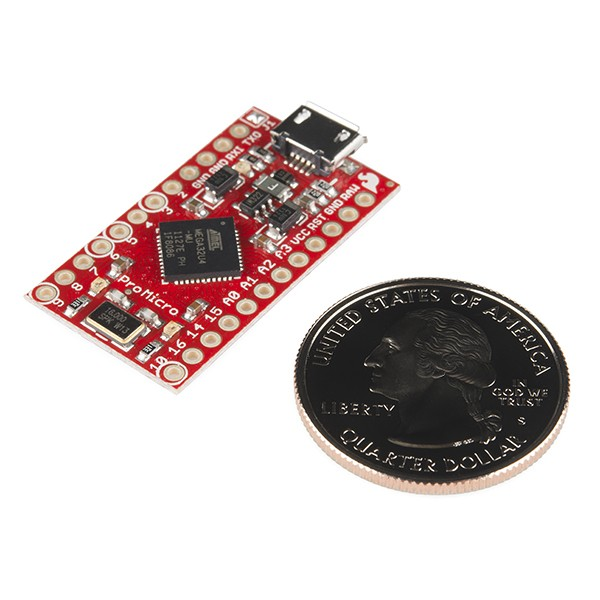
\includegraphics[width=0.7\textwidth]{Chapter03/res/sparkfun_promicro.jpg}
	\caption{Sparkfun Pro Micro 5V/16MHz}
	\label{fig:sparkfun_promicro}
\end{figure}

La scelta di questa board non è casuale, per il progetto ci interessano le seguenti caratteristiche:
\begin{itemize}
	\item ADC per approssimazioni successive a 10 bit, con la possibilità di controllare via software il comportamento dell'ADC, variando così la velocità di campionamento e i tempi del circuito sample-and-hold
	\item Timer configurabili per generare segnali di varia natura, anche di frequenza molto bassa
	\item Controller USB programmabile, così da poter simulare vari tipi di dispositivo (nel caso di OpenLDAT, una porta seriale e un mouse)
	\item Comunicazione via seriale asincrona rispetto all'esecuzione del firmware (entro certi limiti)
	\item Pin GPIO con supporto ad interrupt, pullup, e logica tri-state
	\item Alta disponibilità di cloni poco costosi
	\item Ampiamente documentato, sia dal produttore che dalla community, poiché è completamente compatibile con l'Arduino Leonardo
	\item Dimensioni ridotte, che consentono di creare un dispositivo di dimensioni ragionevoli e che riceve meno interferenze dall'esterno
\end{itemize}

Altre caratteristiche generali del microcontroller 32U4 sono:
\begin{itemize}
	\item Clock a 16MHz, con una velocità tipica di esecuzione delle istruzioni di 16MIPS
	\item 32kB di memoria flash, di cui 28KB disponibili al software e 4KB riservati al bootloader (che può essere rimosso)
	\item 2.5kB di RAM
	\item 1kB di EEPROM
\end{itemize}

Il secondo componente chiave è il sensore di luminosità Everlight ALS-PT19. Si tratta di un fototransistor dai tempi di risposta molto bassi, con una buona linearità, e un costo molto contenuto. Poiché questo componente è SMD ed è estremamente piccolo, è stato scelto di usare il breakout Adafruit ALS-PT19 mostrato in figura \ref{fig:adafruit_pt19}, che monta il sensore e una resistenza da 10k\si{\ohm} su un piccolo PCB, così da poterlo montare facilmente e avere un valore misurabile in tensione anziché in corrente. Variando il valore della resistenza tra il fototransistor e la massa, si regola la sensibilità del sensore (più è alta la resistenza e più è sensibile alla luce).
\begin{figure}[h]
	\centering
	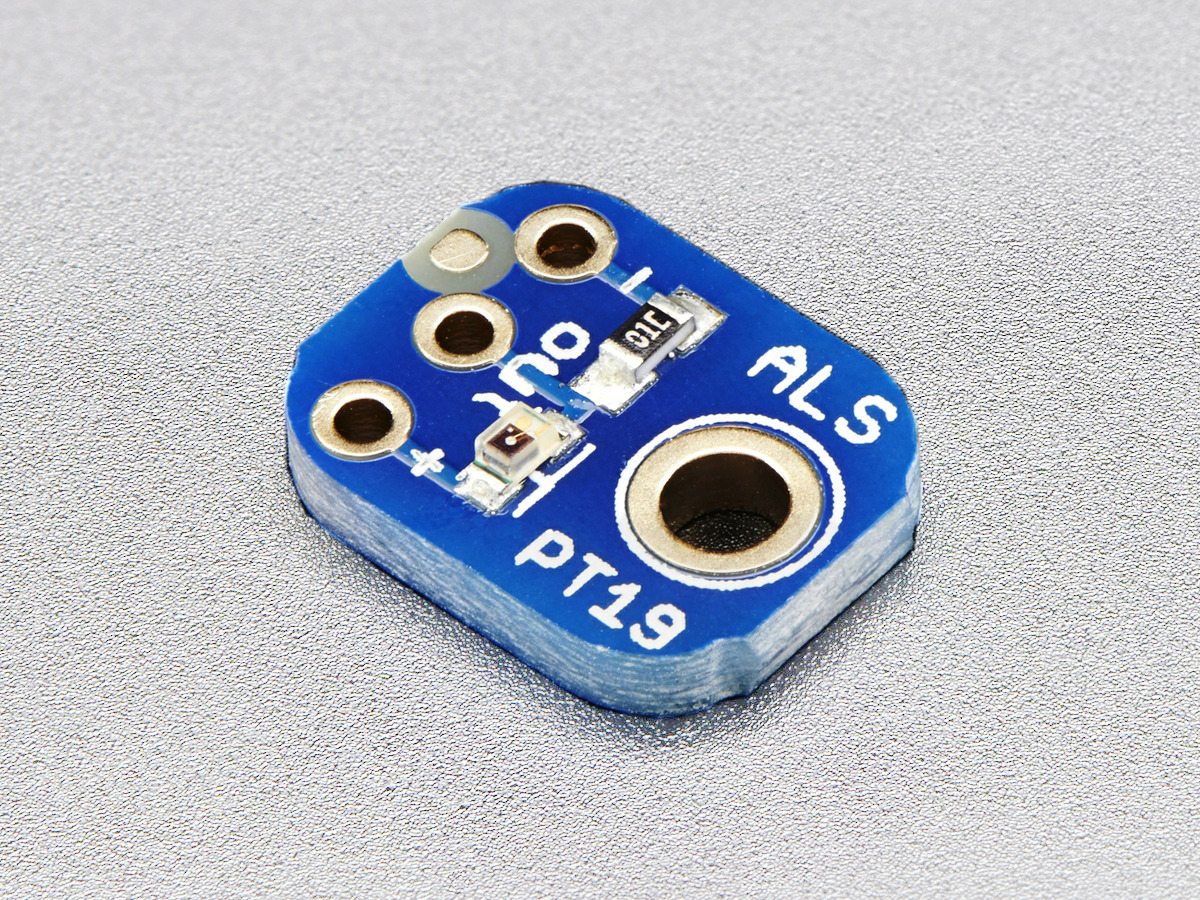
\includegraphics[width=0.7\textwidth]{Chapter03/res/als-pt19.jpg}
	\caption{Adafruit ALS-PT19}
	\label{fig:adafruit_pt19}
\end{figure}

Il sensore ha un tempo di risposta di circa 0.1ms in salita e 0.2ms in discesa \cite{als_pt19_datasheet}, che è stato verificato essere addirittura inferiore collegandolo ad un oscilloscopio, quindi è sufficientemente veloce da poter misurare non solo la latenza totale del sistema, ma anche il comportamento della retroilluminazione e la risposta dei pixel, cosa che non era possibile usando un semplice fotoresistore.

La risposta spettrale del sensore non è particolarmente rilevante per questa applicazione, ma la documentazione mostra una risposta simile a quella dell'occhio umano, con un picco intorno alla lunghezza d'onda del verde \cite{als_pt19_datasheet}, tuttavia è anche sensibile alla luce ultravioletta.

La linearità è importante per questa applicazione. La documentazione del sensore mostra una buona linearità, ma avverte questa è affetta dalla temperatura ambiente e dal voltaggio che viene applicato \cite{als_pt19_datasheet}.\\
Per verificare che la linearità sia sufficiente per lo scopo, è stato realizzato un prototipo dotato del sensore stesso più un sensore AMS TCS34725. Pur non essendo neanche paragonabile ad un colorimetro professionale, questo sensore è calibrato di fabbrica, e la misurazione della luminosità è molto lenta ma più accurata rispetto all'ALS-PT19 \cite{tcs34725_datasheet}.\\
Il grafico in figura \ref{fig:pt19_linearity} mostra sull'asse X la luminosità misurata dal TCS34725, e sull'asse Y quella misurata dall'ALS-PT19 (linea nera). Idealmente dovrebbe essere una linea retta priva di curve (linea rossa).

\begin{figure}[h!]
	\centering
	\begin{tikzpicture}
		\begin{axis}[name=ALS-PT19, xmin=0,xmax=300,ymin=0,ymax=5,width=.7\textwidth,xlabel=Luminosità,ylabel=Voltaggio (V)]
			\addplot[black] file{Chapter03/res/pt19_linearity1.txt};
			\addplot[red] file{Chapter03/res/pt19_linearity2.txt};
		\end{axis}
	\end{tikzpicture}
	\caption{Linearità del sensore ALS-PT19}
	\label{fig:pt19_linearity}
\end{figure}

Il grafico in figura \ref{fig:pt19_linearity3} mostra il rapporto tra la misurazione dell'ALS-PT19 e quella del TCS34725, e permette di vedere meglio che c'è una leggera sovrastima della misura sui valori di luminosità molto bassi, ma poi si stabilizza verso una misura sostanzialmente identica.
\begin{figure}[h!]
	\centering
	\begin{tikzpicture}
		\begin{axis}[name=Rapporto, xmin=0,xmax=300,ymin=0,ymax=2,width=.7\textwidth,xlabel=Luminosità]
			\addplot[black] file{Chapter03/res/pt19_linearity3.txt};
		\end{axis}
	\end{tikzpicture}
	\caption{Rapporto tra ALS-PT19 e TCS34725}
	\label{fig:pt19_linearity3}
\end{figure}

Va inoltre verificato il comportamento man mano che ci si avvicina alla soglia di saturazione. Nella documentazione viene dichiarato che il sensore si comporta linearmente fino alla soglia di saturazione dichiarata di circa 4.75V\cite{als_pt19_datasheet}, ma nella realtà la saturazione comincia a manifestarsi intorno ai 4V, per cui il software deve tenerne conto. Il grafico in figura \ref{fig:pt19_linearity4} mostra la perdita di linearità mentre si avvicina alla soglia di saturazione (Nota: è stata usata una resistenza di alto valore per aumentare il guadagno del sensore).

\begin{figure}[h!]
	\centering
	\begin{tikzpicture}
		\begin{axis}[name=ALS-PT19, xmin=0,xmax=300,ymin=0,ymax=5,width=.7\textwidth,xlabel=Luminosità,ylabel=Voltaggio (V)]
			\addplot[black] file{Chapter03/res/pt19_linearity4.txt};
		\end{axis}
	\end{tikzpicture}
	\caption{Saturazione dell'ALS-PT19}
	\label{fig:pt19_linearity4}
\end{figure}

Questi test sono stati eseguiti leggendo entrambi i sensori contemporaneamente, utilizzando un display in una stanza buia come sorgente luminosa. Il sensore TCS34725 ha il proprio ADC, mentre l'ALS-PT19, essendo un sensore completamente analogico, utilizza uno degli ingressi dell'ADC del microcontroller 32U4. La temperatura ambiente durante i test era di 21°C e il voltaggio applicato ai sensori era 5V. Eventuali errori causati dagli ADC stessi o dalle differenze tra i due ADC non sono misurabili in questo test. Sono stati testati tre ALS-PT19 provenienti da venditori diversi ottenendo risultati virtualmente identici.

\subsection{Schema elettrico}
L'ultimo componente essenziale per il dispositivo OpenLDAT è un circuito (stampato o fatto a mano) che collega tutti i componenti. Questo circuito deve:
\begin{itemize}
	\item Collegare il microcontroller al sensore
	\item Permettere al microcontroller di variare il guadagno del sensore selezionando delle resistenze
	\item Far lampeggiare un LED in corrispondenza ai click (automatici o manuali)
	\item Permettere all'utente di connettere un mouse o un pulsante esterno per generare click manualmente
\end{itemize}

La figura \ref{fig:circuit} mostra lo schema elettrico del circuito che è stato realizzato.
\begin{figure}[h]
	\centering
	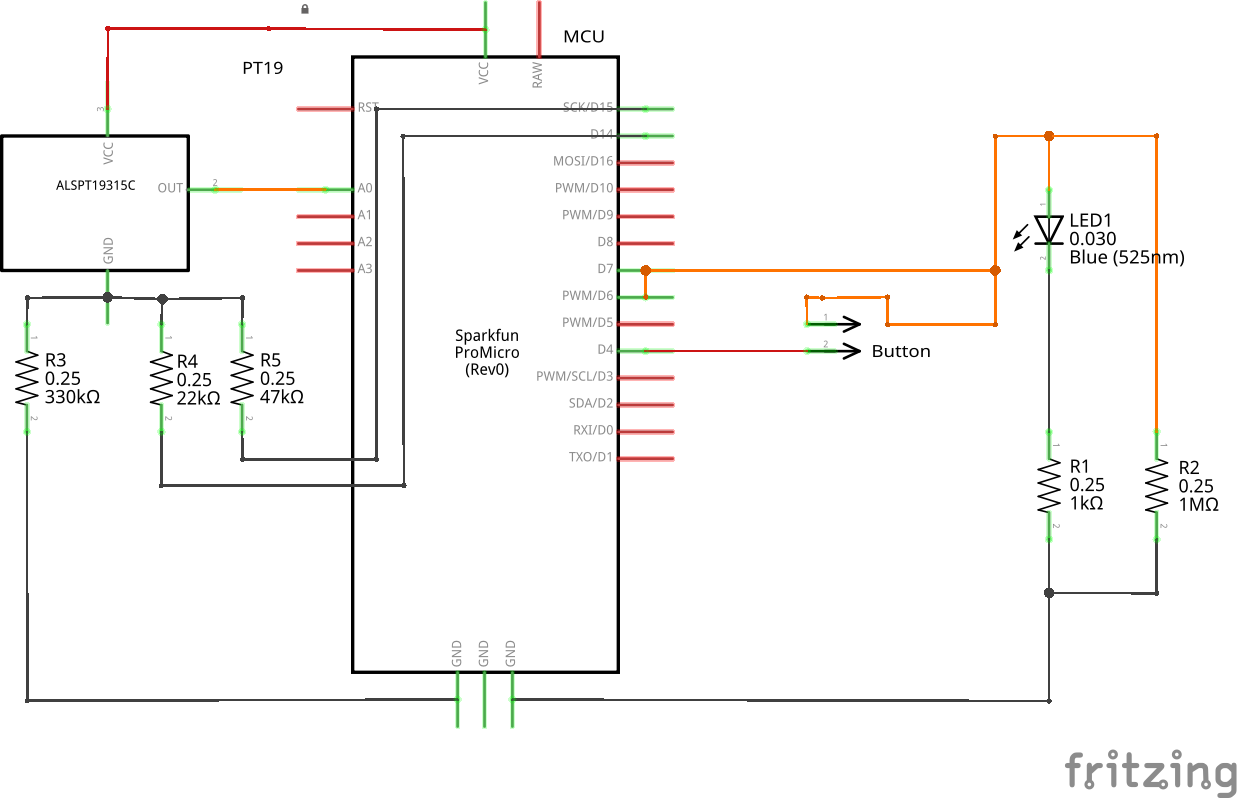
\includegraphics[width=\textwidth]{Chapter03/res/openldat_circuit.png}
	\caption{Schema elettrico del dispositivo OpenLDAT}
	\label{fig:circuit}
\end{figure}

La regolazione del guadagno del sensore avviene mediante le resistenze R3 (330k\si{\ohm}), R4 (22k\si{\ohm}), e R5 (47k\si{\ohm}), posizionate in parallelo in serie alla resistenza da 10k\si{\ohm} già presente sul PCB dell'ALS-PT19. R3 è permanentemente connessa a massa, mentre R4 e R5 possono essere attivate e disattivate controllando lo stato dei pin D14 e D15 rispettivamente. Un pin GPIO in stato \texttt{LOW} equivale ad un collegamento a massa di resistenza trascurabile, mentre un pin in stato \texttt{Z} equivale ad un pin disconnesso (la documentazione del microcontroller indica un'impedenza di 100M\si{\ohm} in questo stato). Svolgendo i calcoli si possono stimare i quattro possibli valori di resistenza davanti al sensore, mostrati in tabella \ref{tab:pt19_gains}. Questi valori sono ovviamente delle stime, e non tengono conto delle tolleranze di produzione delle resistenze e del microcontroller.
\begin{table}
	\centering
	\begin{tabular}{|c|c|c|} 
		\hline
		\textbf{Configurazione (D14,D15)} & \textbf{Resistenza (k\si{\ohm})} & \textbf{Gain relativo}  \\ 
		\hline
		L,L & 24.334   & 1.000         \\ 
		\hline
		Z,L & 30.620   & 1.258         \\ 
		\hline
		L,Z & 51.123   & 2.101         \\ 
		\hline
		Z,Z & 337.847    & 13.883          \\
		\hline
	\end{tabular}
	\caption{\label{tab:pt19_gains}Livelli di gain implementati}
\end{table}

Conoscendo il tipo di luce che genera la retroilluminazione del display (si assume LED con temperatura del bianco neutra), la resistenza usata per il gain, e la precisione dell'ADC, è possibile stimare molto grossolanamente quali sono i livelli di luminosità massima raccomandabili per ogni livello di gain, mostrati in tabella \ref{tab:pt19_nits}. Generalmente i due livelli di gain più elevati sono sufficienti per la maggior parte dei display, mentre quelli più bassi sono utili solo su display HDR.
\begin{table}
	\centering
	\begin{tabular}{|c|c|} 
		\hline
		\textbf{Gain relativo} & \textbf{Luminosità consigliabile (nits)}  \\ 
		\hline
		1.000 & 300-700         \\ 
		\hline
		1.258 & 250-600         \\ 
		\hline
		2.101 & 60-300         \\ 
		\hline
		13.883 & 0-80          \\
		\hline
	\end{tabular}
	\caption{\label{tab:pt19_nits}Range di luminosità del display consigliabile per ogni livello di gain}
\end{table}

La generazione dei click interna e esterna al dispositivo e il lampeggio del LED sono gestiti sulla parte destra dello schema in figura \ref{fig:circuit}. I click vengono captati tramite interrupt sul pin D7. Sfruttando la logica tri-state dei pin GPIO è possibile utilizzare lo stesso circuito per gestire sia i click automatici che quelli manuali:
\begin{itemize}
	\item Quando il dispositivo genera autonomamente i click, un timer interno al microcontroller manda brevi pulsazioni a una frequenza di circa 1Hz dal pin D6, e quindi varia tra gli stati \texttt{HIGH} e \texttt{LOW}, mentre il pin D4 è posizionato in stato \texttt{Z}, come se fosse disconnesso. Quando il segnale dal pin D6 passa ad \texttt{HIGH}, D7 riceve l'interrupt, e contemporaneamente si accende il LED. I pin per il pulsante sono inattivi in questa modalità, e cortocircuitarli non ha alcun effetto sul dispositivo
	\item Quando il dispositivo riceve i click dall'esterno, il pin D4 è in stato \texttt{HIGH} per fornire alimentazione al pulsante esterno, mentre il pin D6 è in stato Z, come se fosse disconnesso. Quando il pulsante esterno viene premuto, i due contatti per il pulsante vengono cortocircuitati, D7 riceve l'interrupt, e contemporaneamente si accende il LED
\end{itemize}

La resistenza R1 serve per limitare la luminosità del LED, mentre la resistenza R2 fa da pull-down per evitare che il pin D7 vada in stato floating quando si ricevono i click dall'esterno e il pulsante esterno non è premuto.

Poiché il lampeggio del LED è gestito in modo totalmente analogico, non c'è ritardo introdotto dal firmware.

\subsection{PCB}
Il circuito può essere stampato su un PCB a singolo strato delle dimensioni di 23x41mm e uno spessore di 1.6mm, su cui poi si saldano i componenti. Il PCB è pensato per essere semplice da realizzare anche in casa se si hanno gli strumenti per farlo, non è necessario utilizzare servizi di produzione professionali.

La figura \ref{fig:pcb} mostra due viste del PCB da sopra e da sotto: sul lato superiore sono presenti la board con il microcontroller, i pin per il mouse esterno e il LED, mentre sul lato inferiore sono presenti il breakout con il sensore ALS-PT19 e le varie resistenze per controllarne il gain. Tutte le piste che collegano i componenti sono sul lato inferiore.
\begin{figure}[h]
	\centering
	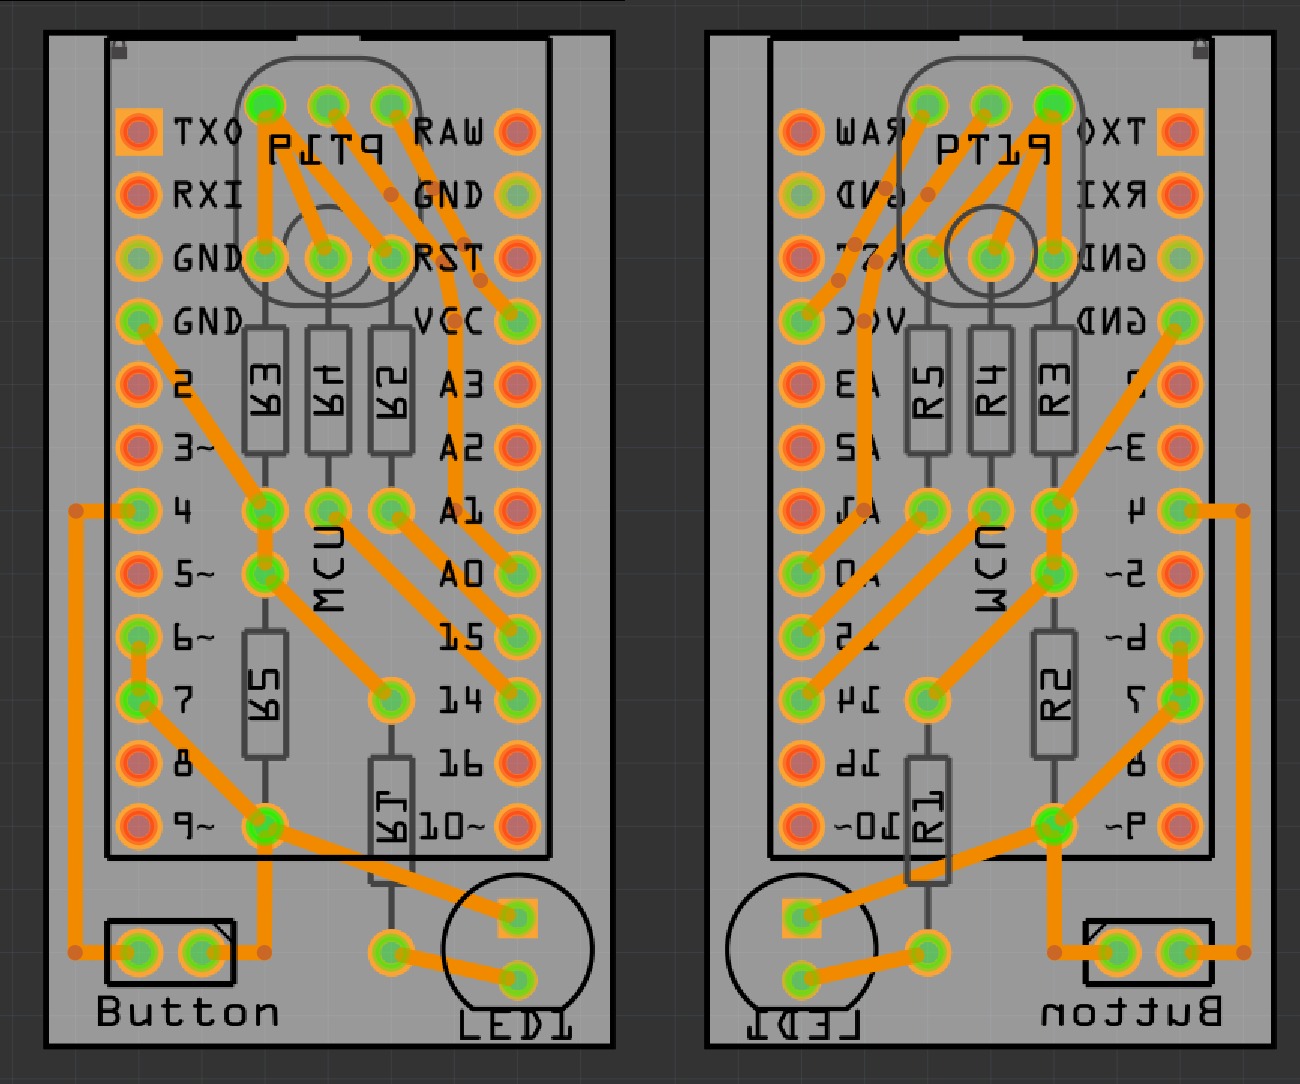
\includegraphics[width=\textwidth]{Chapter03/res/openldat_pcb.png}
	\caption{Il PCB del dispositivo OpenLDAT visto da sopra e da sotto}
	\label{fig:pcb}
\end{figure}

\subsection{Case}
È stato realizzato un case per il dispositivo stampabile con una stampante 3D, progettato per essere facile da stampare e montare, che minimizzi le infiltrazioni di luce indesiderate, e che permetta di appoggiare il dispositivo sullo schermo da testare senza rischiare di graffiarne il vetro.

Il case è composto da tre parti (di cui una opzionale):
\begin{itemize}
	\item La base (figura \ref{fig:case_base}): è la parte principale, dalla forma circolare con un diametro di 59mm e un'altezza di 21mm, con quattro supporti in cui incastrare il PCB, due supporti laterali in cui incastrare il coperchio, un foro di 14x14mm sulla parte inferiore dove può passare la luce verso il sensore, e uno sul lato per la porta USB. Attorno al foro per il sensore è presente un piccolo incavo in cui è possibile, opzionalmente, incollare un vetrino da microscopio 22x22mm per proteggere il sensore. Sempre opzionalmente, è possibile posizionare dei feltrini sottili o del velluto sulla parte che si appoggia sullo schermo, per un'ulteriore protezione contro graffi accidentali
	\item Il coperchio (figura \ref{fig:case_top}): si incastra nei due supporti laterali e permette di bloccare la luce dall'esterno. Due fori consentono il collegamento del pulsante esterno e rendono visibile il LED sul dispositivo, due barrette tengono fermo il PCB, qualora dovesse uscire dagli incastri della base
	\item Diffusore per il LED (figura \ref{fig:case_ledcover}): un piccolo pezzo di plastica trasparente, del tutto opzionale, che può essere incastrato nel foro per il LED presente sul coperchio, così da rendere più esteticamente piacevole la luce del LED del dispositivo. Rende inoltre visibile la luce dei LED sulla board del microcontroller, che si illuminano durante la comunicazione con il PC
\end{itemize}

Se stampato correttamente, la distribuzione del peso del case stesso gli permette di stare fermo quando è appoggiato al display.

\begin{figure}[H]
	\centering
	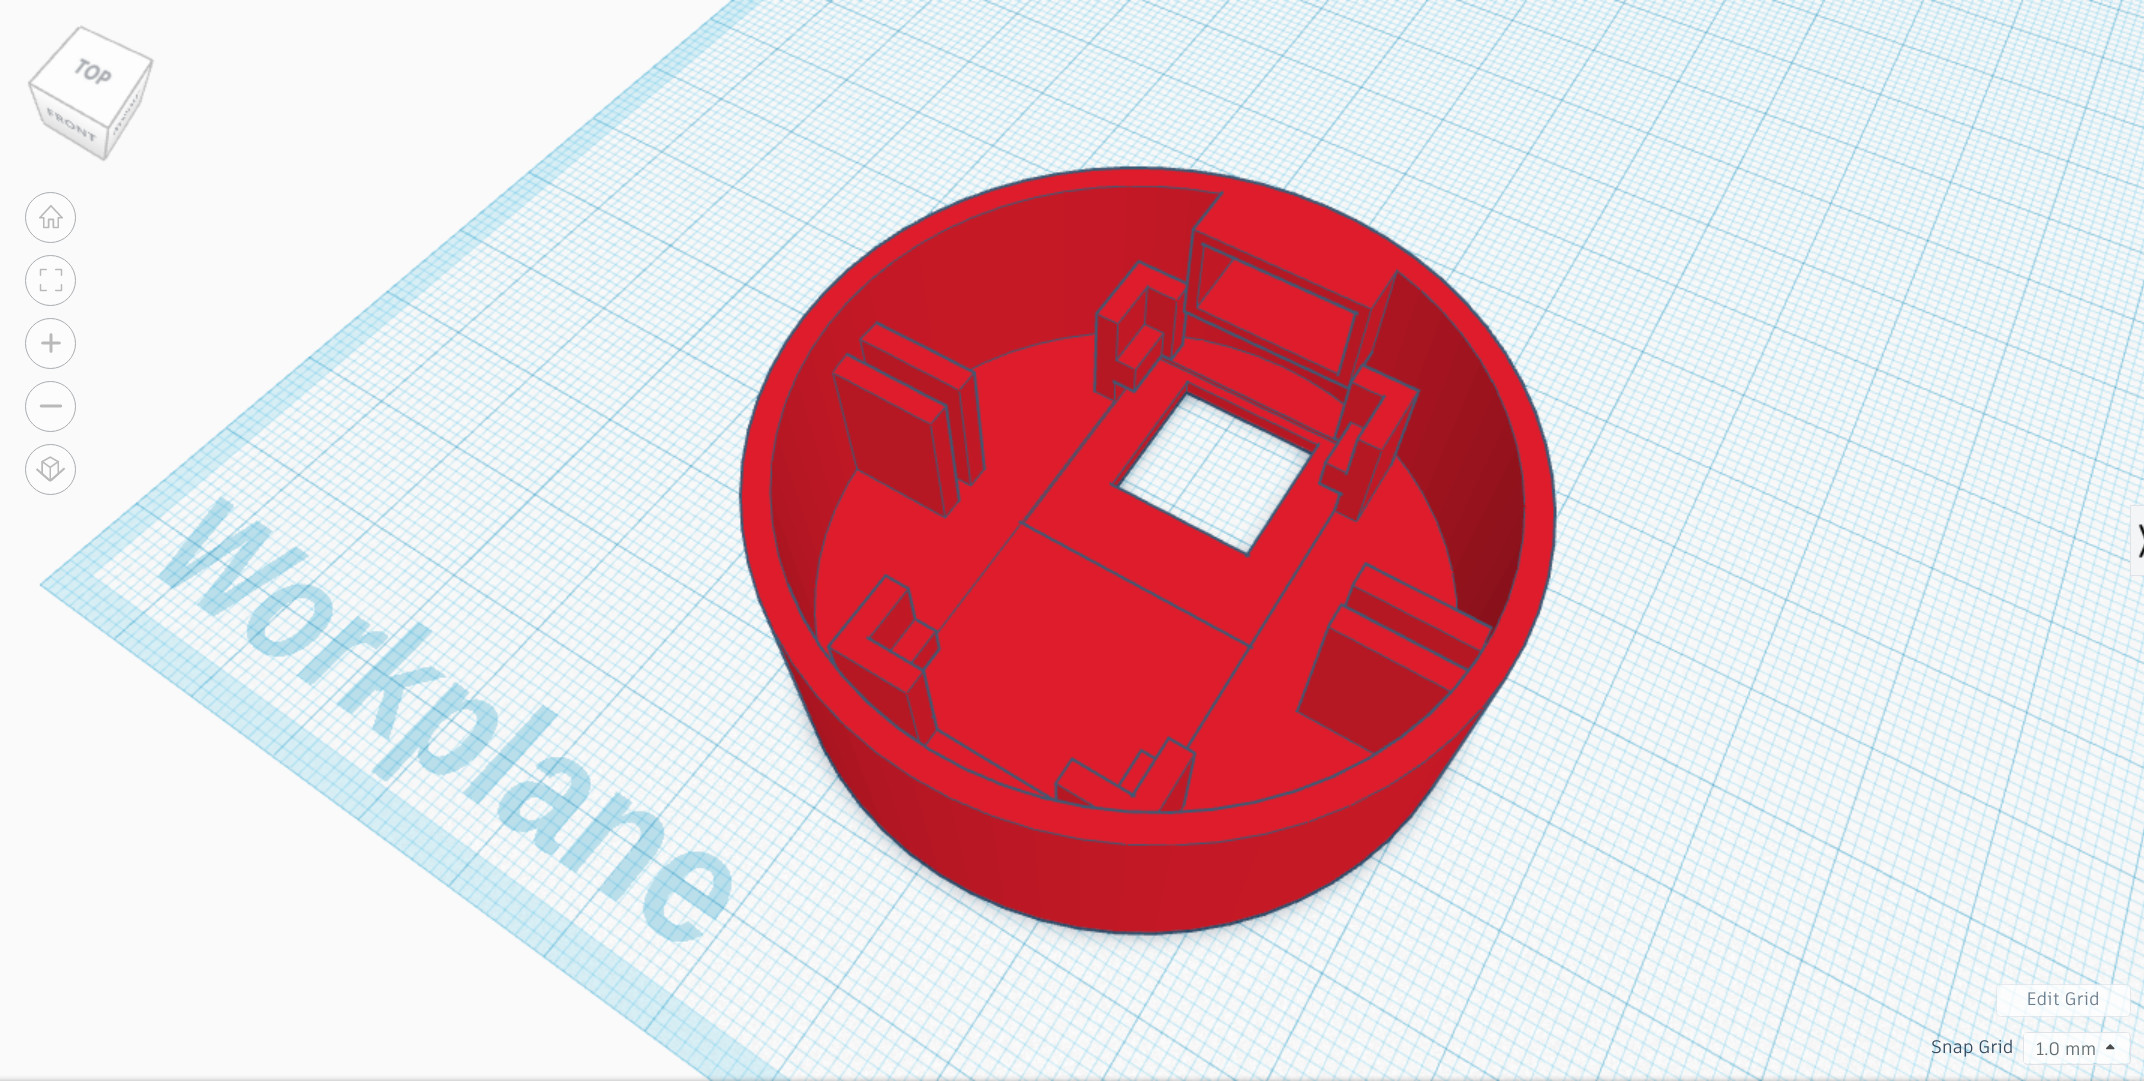
\includegraphics[width=\textwidth]{Chapter03/res/openldat_case_base1.jpg}
	\caption{Base del case}
	\label{fig:case_base}
\end{figure}
\begin{figure}[H]
	\centering
	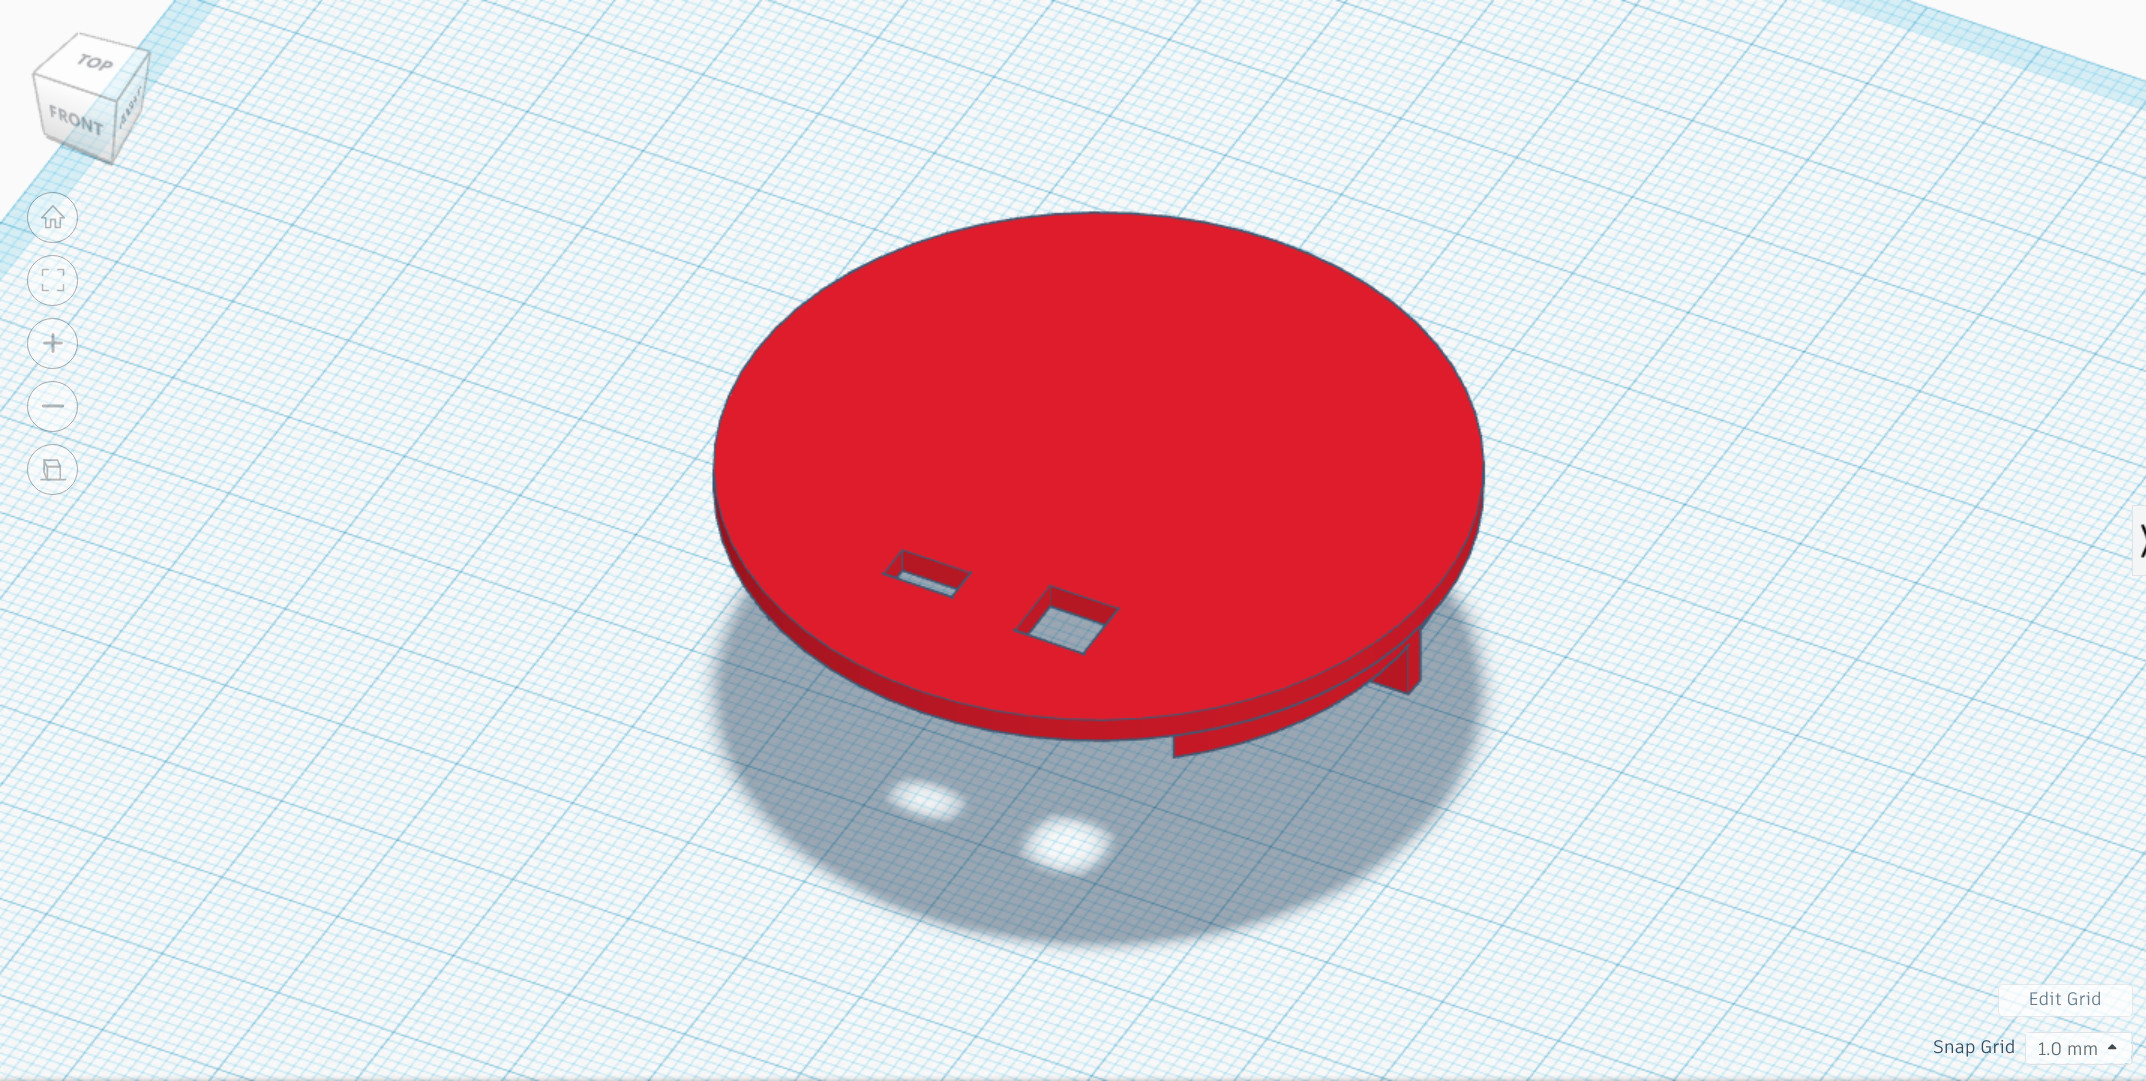
\includegraphics[width=\textwidth]{Chapter03/res/openldat_case_top1.jpg}
	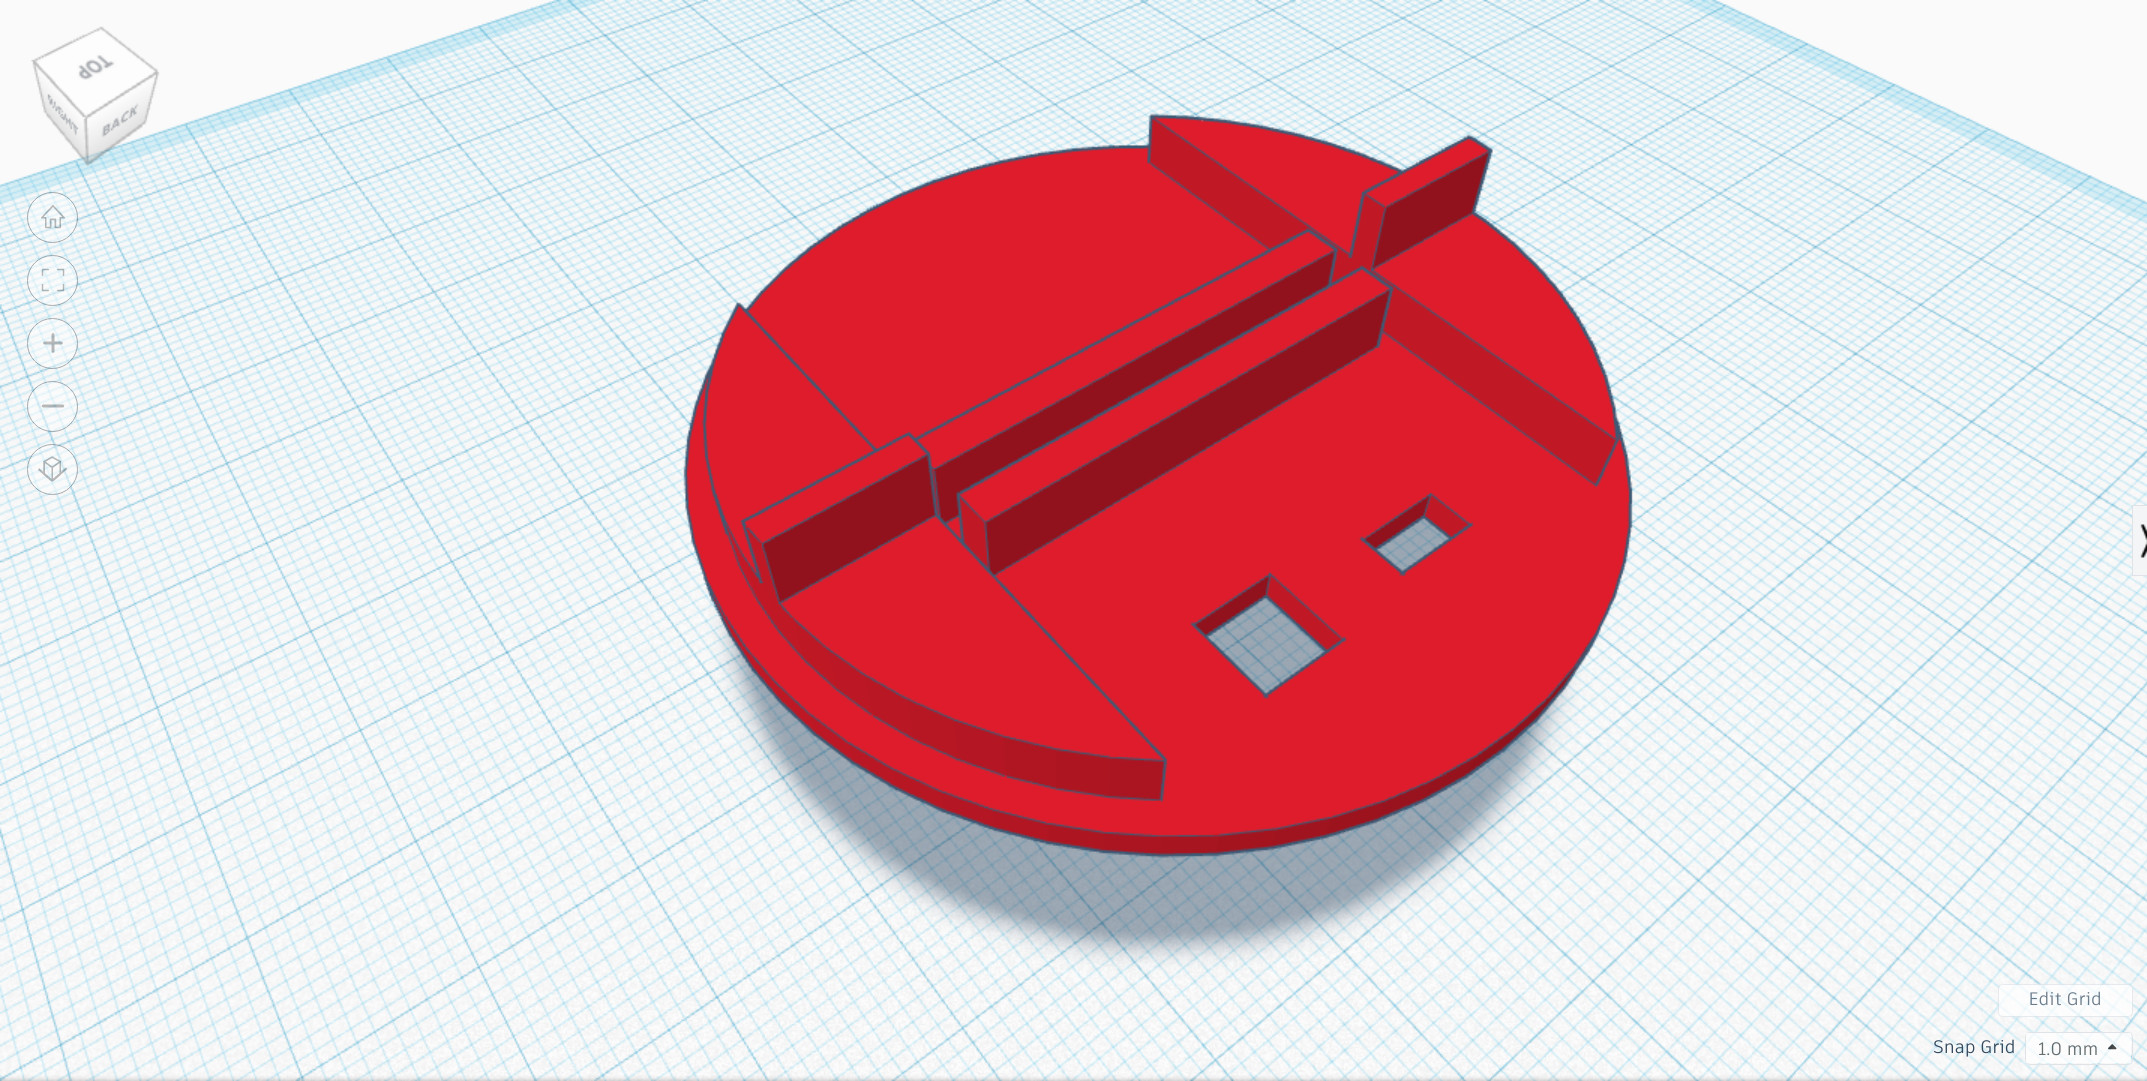
\includegraphics[width=\textwidth]{Chapter03/res/openldat_case_top2.jpg}
	\caption{Coperchio del case}
	\label{fig:case_top}
\end{figure}
\begin{figure}[H]
	\centering
	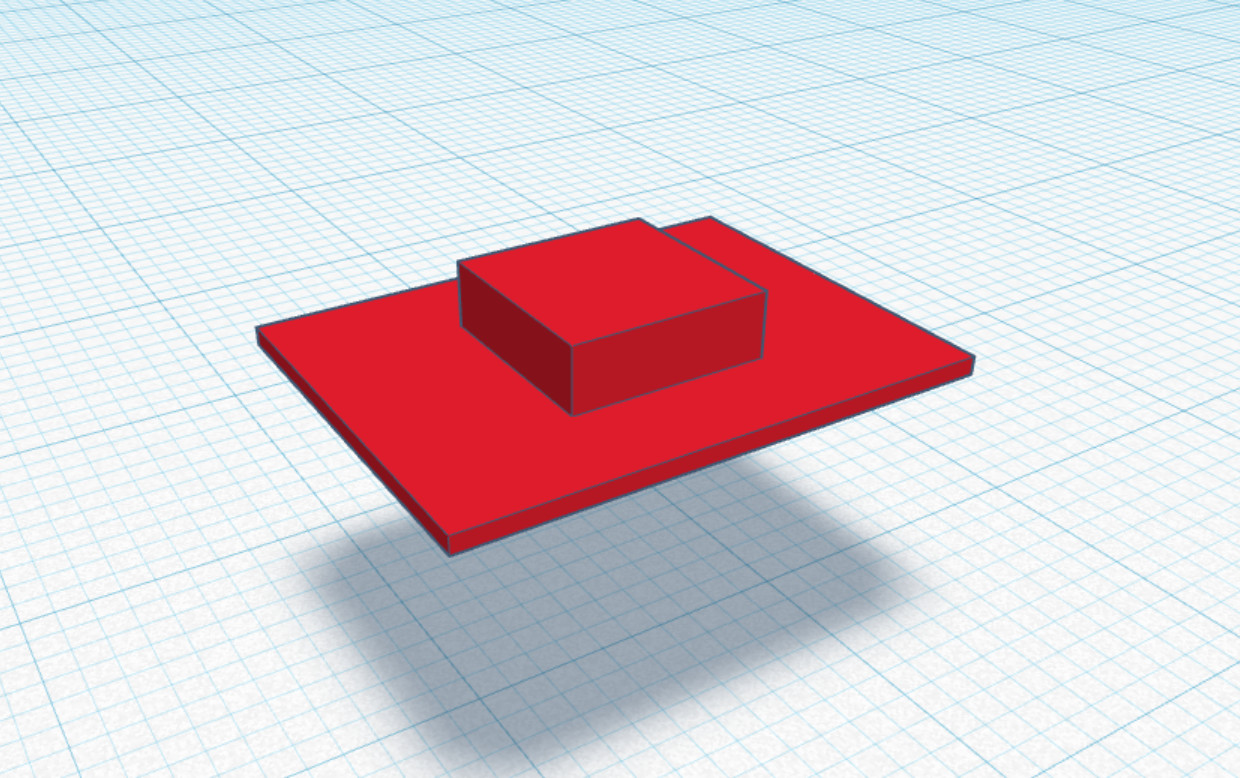
\includegraphics[width=\textwidth]{Chapter03/res/openldat_case_ledcover.jpg}
	\caption{Diffusore trasparente per il LED (opzionale)}
	\label{fig:case_ledcover}
\end{figure}

\subsection{Bill Of Materials}
La tabella \ref{tab:bom} mostra tutto il materiale necessario per costruire il dispositivo OpenLDAT. I prezzi sono aggiornati a Aprile 2021 e variano molto a seconda delle quantità ordinate (la tabella fa riferimento a un ordine per i componenti per assemblare 9-10 dispositivi). Non tutti i componenti sono essenziali.

\begin{table}[h!]
	\centering
	\resizebox{\columnwidth}{!}{\begin{tabular}{|l|l|l|l|} 
		\hline
		\textbf{Essenziale} & \textbf{Nome} & \textbf{Fornitore} & \textbf{Prezzo (€)}  \\ 
		\hline
		Si & Sparkfun Pro Micro 5V/16MHz (clone) con header & Aliexpress (keyword: 32u4) & 4.98         \\ 
		\hline
		Si & Adafruit ALS-PT19 con header & Aliexpress (keyword: als pt19) & 2.28         \\
		\hline
		Si & PCB OpenLDAT & Aisler & 2.45        \\
		\hline
		Si & Resistenze ¼W: 1M\si{\ohm}, 1k\si{\ohm}, 330k\si{\ohm}, 22k\si{\ohm}, 47k\si{\ohm} & Qualsiasi & 0.10        \\
		\hline
		Si & 2 pin header maschio & Inclusi col sensore & 0.00\\
		\hline
		Si & LED 3mm (qualsiasi colore) & Qualsiasi & 0.02 \\
		\hline
		No & 50g PLA Nero & Amazon (marca GIANTARM) & 0.90        \\
		\hline
		No & 2g PLA Trasparente & Amazon (marca GIANTARM) & 0.04        \\
		\hline
		No & Vetrino coprioggetto per microscopio 22x22mm & Amazon & 0.05        \\
		\hline
	\end{tabular}}
	\caption{\label{tab:bom}Materiali per la realizzazione il dispositivo OpenLDAT}
\end{table}

\subsection{Costruzione del mouse modificato}
Per misurare la latenza di una macchina separata è necessario modificare un mouse (o volendo un controller) in modo che quando viene premuto il tasto per fare fuoco vengano cortocircuitati i due pin per il pulsante esterno sul dispositivo OpenLDAT. Eseguire questa modifica richiede un minimo di competenze elettroniche poiché ogni modello di mouse è diverso: nei casi più semplici è possibile collegare i contatti del pulsante ai pin del dispositivo, ma più in generale è consigliabile l'uso di un analog switch come l'integrato Vishay DG213DJ\cite{vishay_dg213_datasheet}, il quale può essere alimentato direttamente dal mouse, può gestire sia segnali normalmente alti che normalmente bassi, e può cortocircuitare i pin del pulsante esterno in risposta ai click in totale sicurezza.\\
Sul dispositivo OpenLDAT, il pin di sinistra porta un segnale \texttt{HIGH} (5V), mentre il pin di destra è in alta impedenza in attesa di ricevere il segnale. La soglia di attivazione del pin di destra è circa 3V\cite{atmega32u4_datasheet}. La quantità di corrente che può passare è limitata a pochi mA dal LED e dalle resistenze presenti tra il pin di destra e la massa.\\
Il circuito in figura \ref{fig:modmouse_example} mostra un esempio di circuito per un mouse modificato, ma potrebbe variare molto tra mouse diversi: potrebbe essere necessario cambiare o rimuovere la resistenza in input o creare un pull-up/pull-down, o costruire un circuito totalmente diverso.

\begin{figure}[h!]
	\centering
	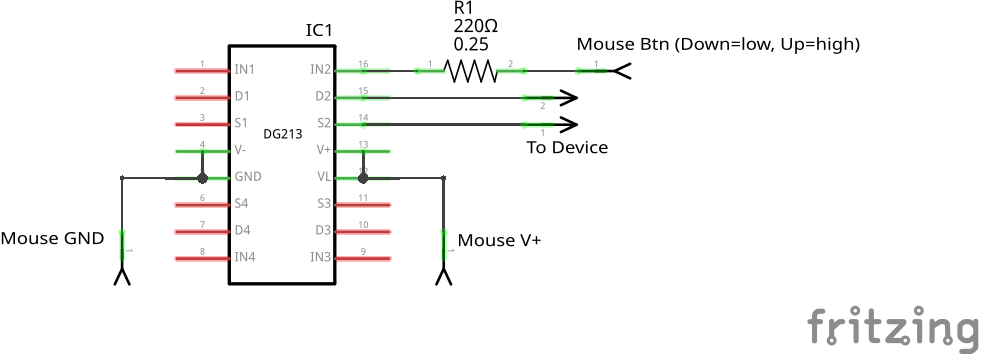
\includegraphics[width=\textwidth]{Chapter03/res/modmouse_example.png}
	\caption{Esempio di circuito per mouse modificato}
	\label{fig:modmouse_example}
\end{figure}

Una volta assemblato, il circuito può essere nascosto all'interno del mouse, lasciando uscire solo i cavi da connettere sul dispositivo OpenLDAT.

Attenzione: un circuito errato potrebbe danneggiare permanentemente il dispositivo OpenLDAT e/o il mouse.
